\documentclass[answers]{exam}

\usepackage{graphicx}
\usepackage{float}
\usepackage{amsmath}
\usepackage{subcaption}
\usepackage{framed}
\usepackage{amsthm}
\usepackage{amsmath}
\usepackage{amsfonts}
\usepackage{algorithmicx}
\usepackage{algpseudocode}
\usepackage{mathtools}
\usepackage{tikz}
\newcommand\numberthis{\addtocounter{equation}{1}\tag{\theequation}}
\newtheorem{lemma}{Lemma}
\newtheorem{claim}{Claim}
\usepackage{etoolbox}
\AtBeginEnvironment{solution}{\setcounter{claim}{0}}

\usetikzlibrary{fit}
\usetikzlibrary{arrows}
\newcommand\addvmargin[1]{
  \node[fit=(current bounding box),inner ysep=#1,inner xsep=0]{};
}

\DeclareMathOperator*{\argmax}{arg\,max}

\newcommand{\nl}{\vspace{0.2cm}\\}
\newcommand{\nln}{\vspace{0.2cm}}

% First we setup the header and footer
\pagestyle{headandfoot}
\runningheadrule
\runningfootrule
\header{COL351: Analysis and Design of Algorithms (CSE, IITD, Semester-I-2020-21)}{}{Homework-5}
\footer{}{\thepage  \, of \numpages}{}
 
% We want the points for each question displayed on the left
%\pointname{points}
%\pointsinmargin
 
% Automatically total the points - make sure to compile TWICE
\addpoints
 
\begin{document}


\begin{center} 
\fbox{\parbox{5.5in}{
\vspace{-0.1in}
\begin{itemize}
\item \small{The instructions are the same as in Homework-0, 1, 2.}
\end{itemize}
\vspace{-0.1in}
}}
\end{center}

\vspace{0.1in}


\vspace{0.1in}
% Some general text together with number of questions and total points possible
There are \numquestions\, questions for a total of \numpoints\, points.
\vspace{0.1in}
\hrule
 \vspace{0.2in}
\begin{questions}
 
% First question, worth 3 points
\question[20] Consider the network shown in the figure. Consider running the Ford-Fulkerson algorithm on this network. 
\begin{figure}[h]
\centering
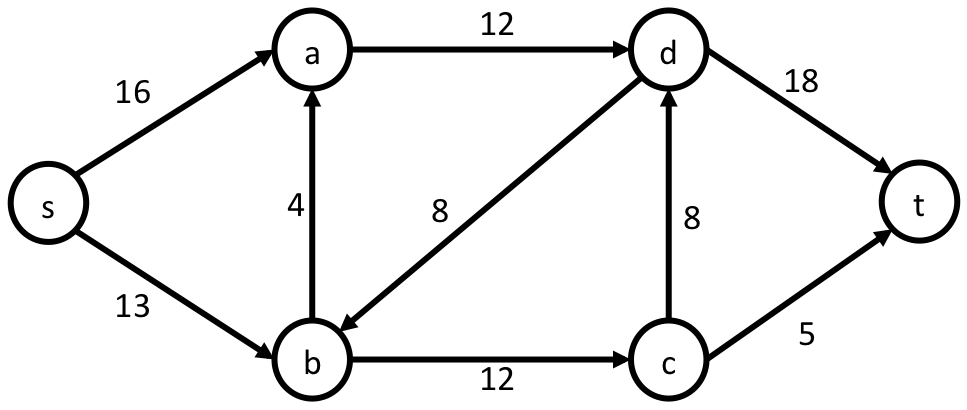
\includegraphics[scale=0.25]{embed/network-1}
\end{figure}

\begin{parts}
\part We start with a zero $s$-$t$ flow $f$. The algorithm then finds an augmenting path in $G_f$. Suppose the augmenting path is $s \rightarrow b \rightarrow c \rightarrow t$. Give the flow $f'$ after augmenting flow along this path.
\begin{solution}

A flow is a function from edges to non-negative real numbers, so it suffices to give the flow value for each edge.

$f'((s,b))=5,$ $f'((s,a))=0,$ $f'((b,a))=0,$ $f'((a,d))=0,$ $f'((d,b))=0,$ $f'((b,c))=5,$ $f'((c,d))=0,$ $f'((c,t))=5,$ $f'((d,t))=0$
\end{solution}

\part Show the graph $G_{f'}$. That is, the residual graph with respect to $s$-$t$ flow $f'$.
\begin{solution}

In all the following parts, back edges that are not drawn should be treated to have zero weight. This has been done for the sake of a clear diagram (and as clarified on Piazza, it is valid too).

%\begin{figure}[H]
%\centering
%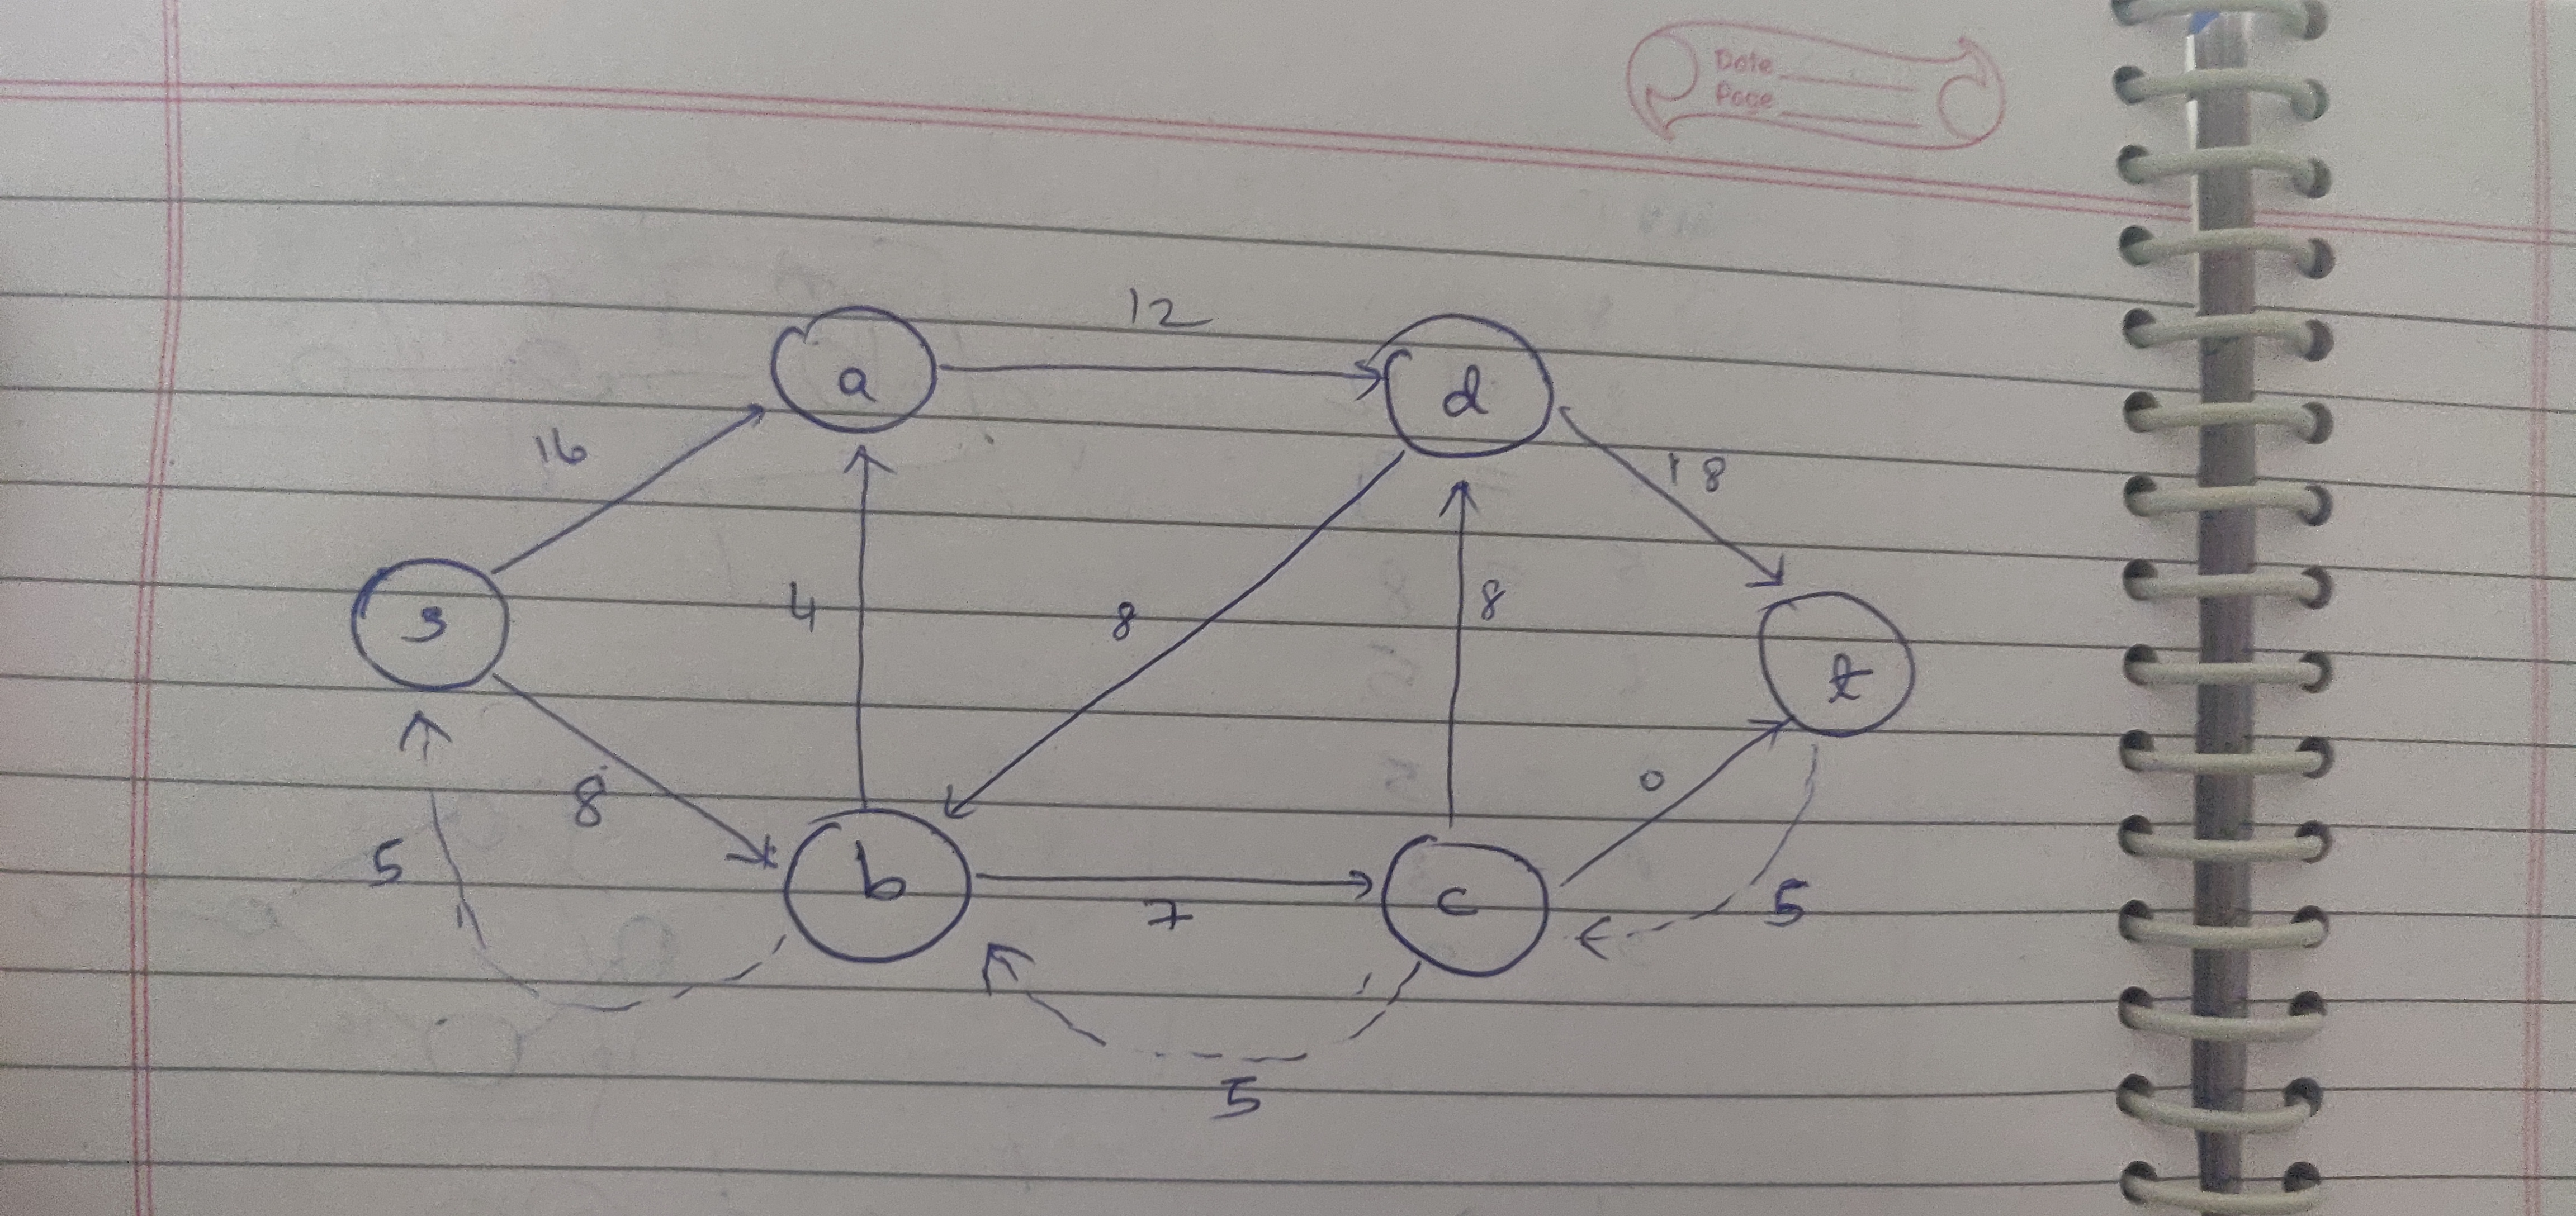
\includegraphics[scale=0.085]{1_a.jpg}
%\end{figure}

\begin{center}
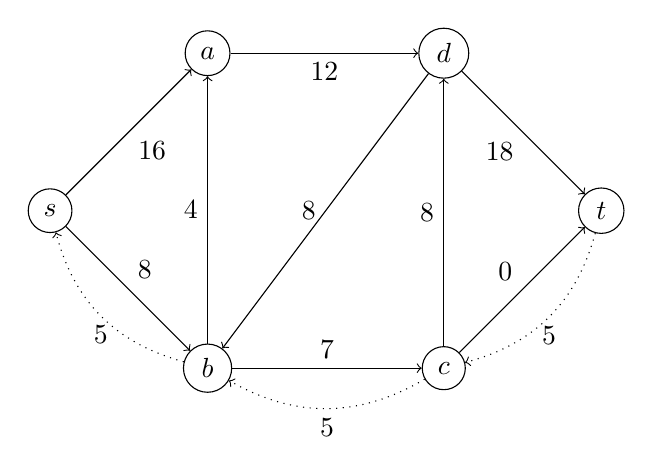
\begin{tikzpicture}
\tikzset{vertex/.style = {shape=circle,draw,minimum size=1.5em}}
\tikzset{edge/.style = {->,> = latex'}}
\node[vertex](s) at (0, 0) {$s$};
\node[vertex](a) at (2, 2) {$a$};
\node[vertex](b) at (2, -2) {$b$};
\node[vertex](c) at (5, -2) {$c$};
\node[vertex](d) at (5, 2) {$d$};
\node[vertex](t) at (7, 0) {$t$};
\draw[->] (s) -- (a) node[midway, below right] {$16$};
\draw[->] (s) -- (b) node[midway, above right] {$8$};
\draw[->] (b) -- (a) node[midway, left] {$4$};
\draw[->] (a) -- (d) node[midway, below] {$12$};
\draw[->] (d) -- (b) node[midway, left] {$8$};
\draw[->] (b) -- (c) node[midway, above] {$7$};
\draw[->] (c) -- (d) node[midway, left] {$8$};
\draw[->] (c) -- (t) node[midway, above left] {$0$};
\draw[->] (d) -- (t) node[midway, below left] {$18$};
\draw[->, dotted] (b) to [bend left] node[midway, below] {$5$} (s);
\draw[->, dotted] (c) to [bend left] node[midway, below] {$5$} (b);
\draw[->, dotted] (t) to [bend left] node[midway, below] {$5$} (c);
\end{tikzpicture}
\end{center}

\end{solution}

\part The algorithm then sets $f$ as $f'$ and $G_f$ as $G_{f'}$ and repeats. Suppose the augmenting path chosen in the next iteration of the while loop is $s \rightarrow a \rightarrow d \rightarrow t$. Give $f'$ after augmenting flow along this path and show $G_{f'}$.
\begin{solution}
$f'((s,b))=5,$ $f'((s,a))=12,$ $f'((b,a))=0,$ $f'((a,d))=12,$ $f'((d,b))=0,$ $f'((b,c))=5,$ $f'((c,d))=0,$ $f'((c,t))=5,$ $f'((d,t))=12$

%\begin{figure}[H]
%\centering
%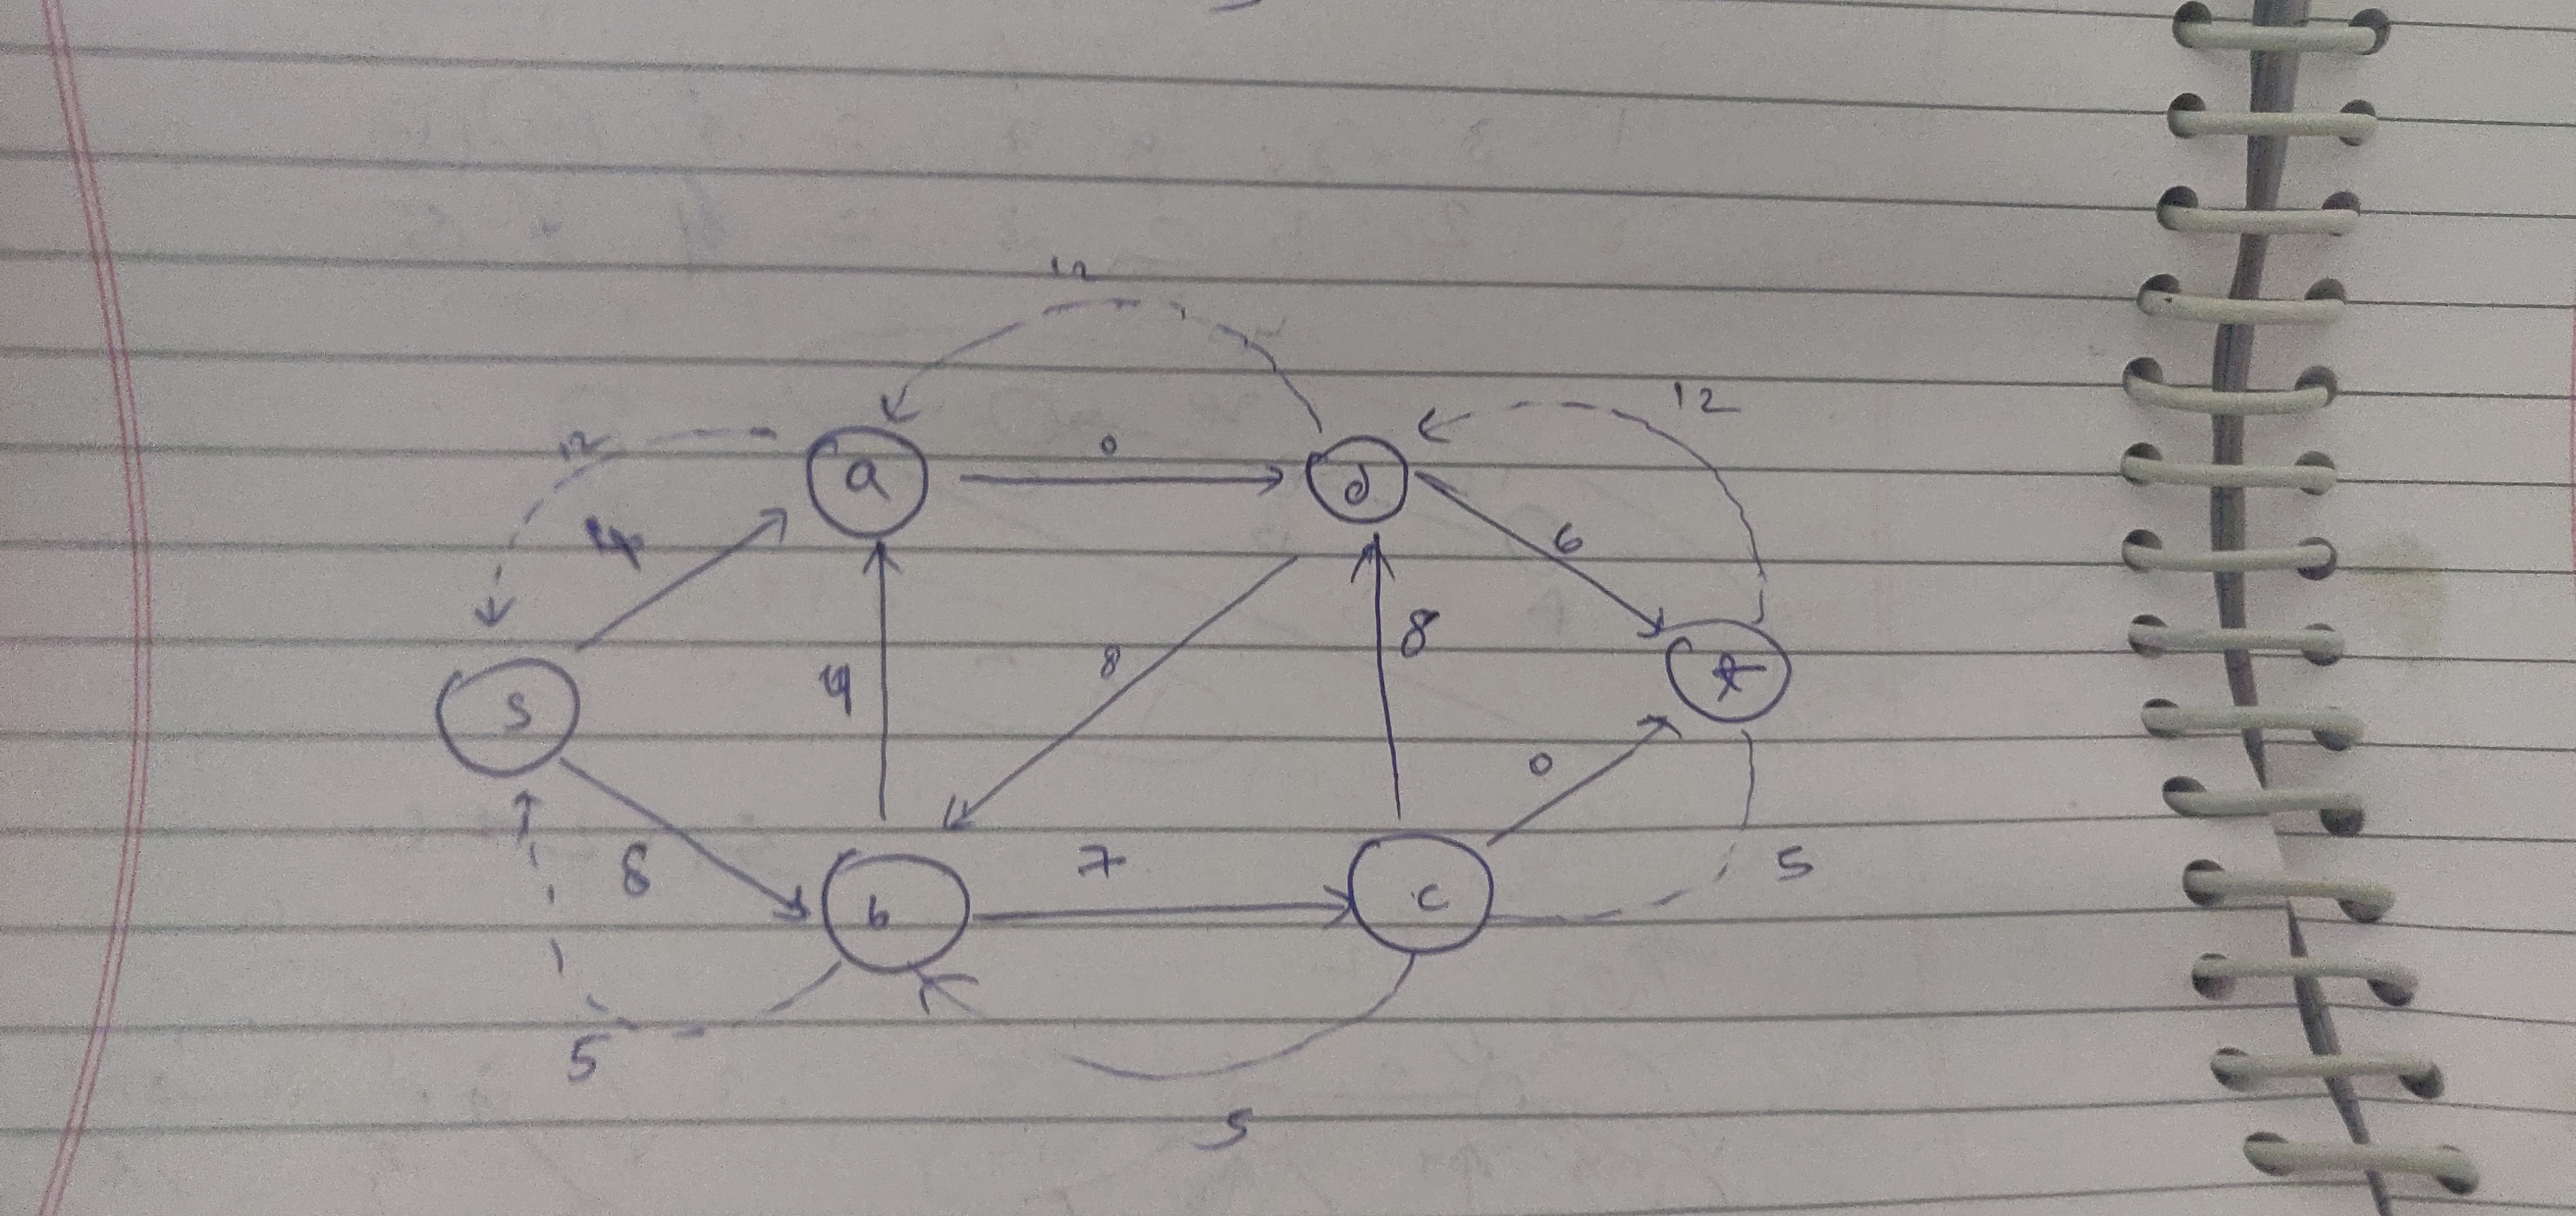
\includegraphics[scale=0.085]{1_b.jpg}
%\end{figure}

\begin{center}
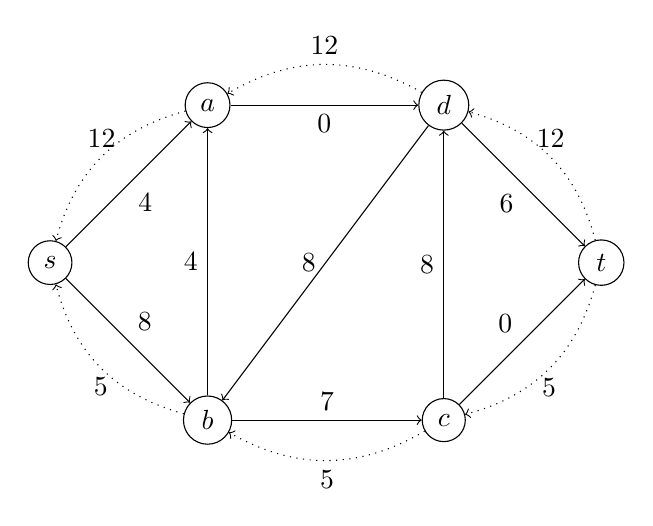
\begin{tikzpicture}
\tikzset{vertex/.style = {shape=circle,draw,minimum size=1.5em}}
\tikzset{edge/.style = {->,> = latex'}}
\node[vertex](s) at (0, 0) {$s$};
\node[vertex](a) at (2, 2) {$a$};
\node[vertex](b) at (2, -2) {$b$};
\node[vertex](c) at (5, -2) {$c$};
\node[vertex](d) at (5, 2) {$d$};
\node[vertex](t) at (7, 0) {$t$};
\draw[->] (s) -- (a) node[midway, below right] {$4$};
\draw[->] (s) -- (b) node[midway, above right] {$8$};
\draw[->] (b) -- (a) node[midway, left] {$4$};
\draw[->] (a) -- (d) node[midway, below] {$0$};
\draw[->] (d) -- (b) node[midway, left] {$8$};
\draw[->] (b) -- (c) node[midway, above] {$7$};
\draw[->] (c) -- (d) node[midway, left] {$8$};
\draw[->] (c) -- (t) node[midway, above left] {$0$};
\draw[->] (d) -- (t) node[midway, below left] {$6$};
\draw[->, dotted] (b) to [bend left] node[midway, below] {$5$} (s);
\draw[->, dotted] (c) to [bend left] node[midway, below] {$5$} (b);
\draw[->, dotted] (t) to [bend left] node[midway, below] {$5$} (c);
\draw[->, dotted] (a) to [bend right] node[midway, above] {$12$} (s);
\draw[->, dotted] (d) to [bend right] node[midway, above] {$12$} (a);
\draw[->, dotted] (t) to [bend right] node[midway, above] {$12$} (d);
\end{tikzpicture}
\end{center}


\end{solution}

\part Let $f$ be the flow when the algorithm terminates. Give the flow $f$ and draw the residual graph $G_f$.
\begin{solution}

The residual graph has two augmenting paths: $s \to b \to d \to t$ and $s \to b \to c \to d \to t$, and after taking either of these two, the algorithm terminates. We suppose that the second augmenting path is chosen.

$f((s,b))=11,$ $f((s,a))=12,$ $f((b,a))=0,$ $f((a,d))=12,$ $f((d,b))=0,$ $f((b,c))=11,$ $f((c,d))=6,$ $f'((c,t))=5,$ $f((d,t))=18$
%\begin{figure}[H]
%\centering
%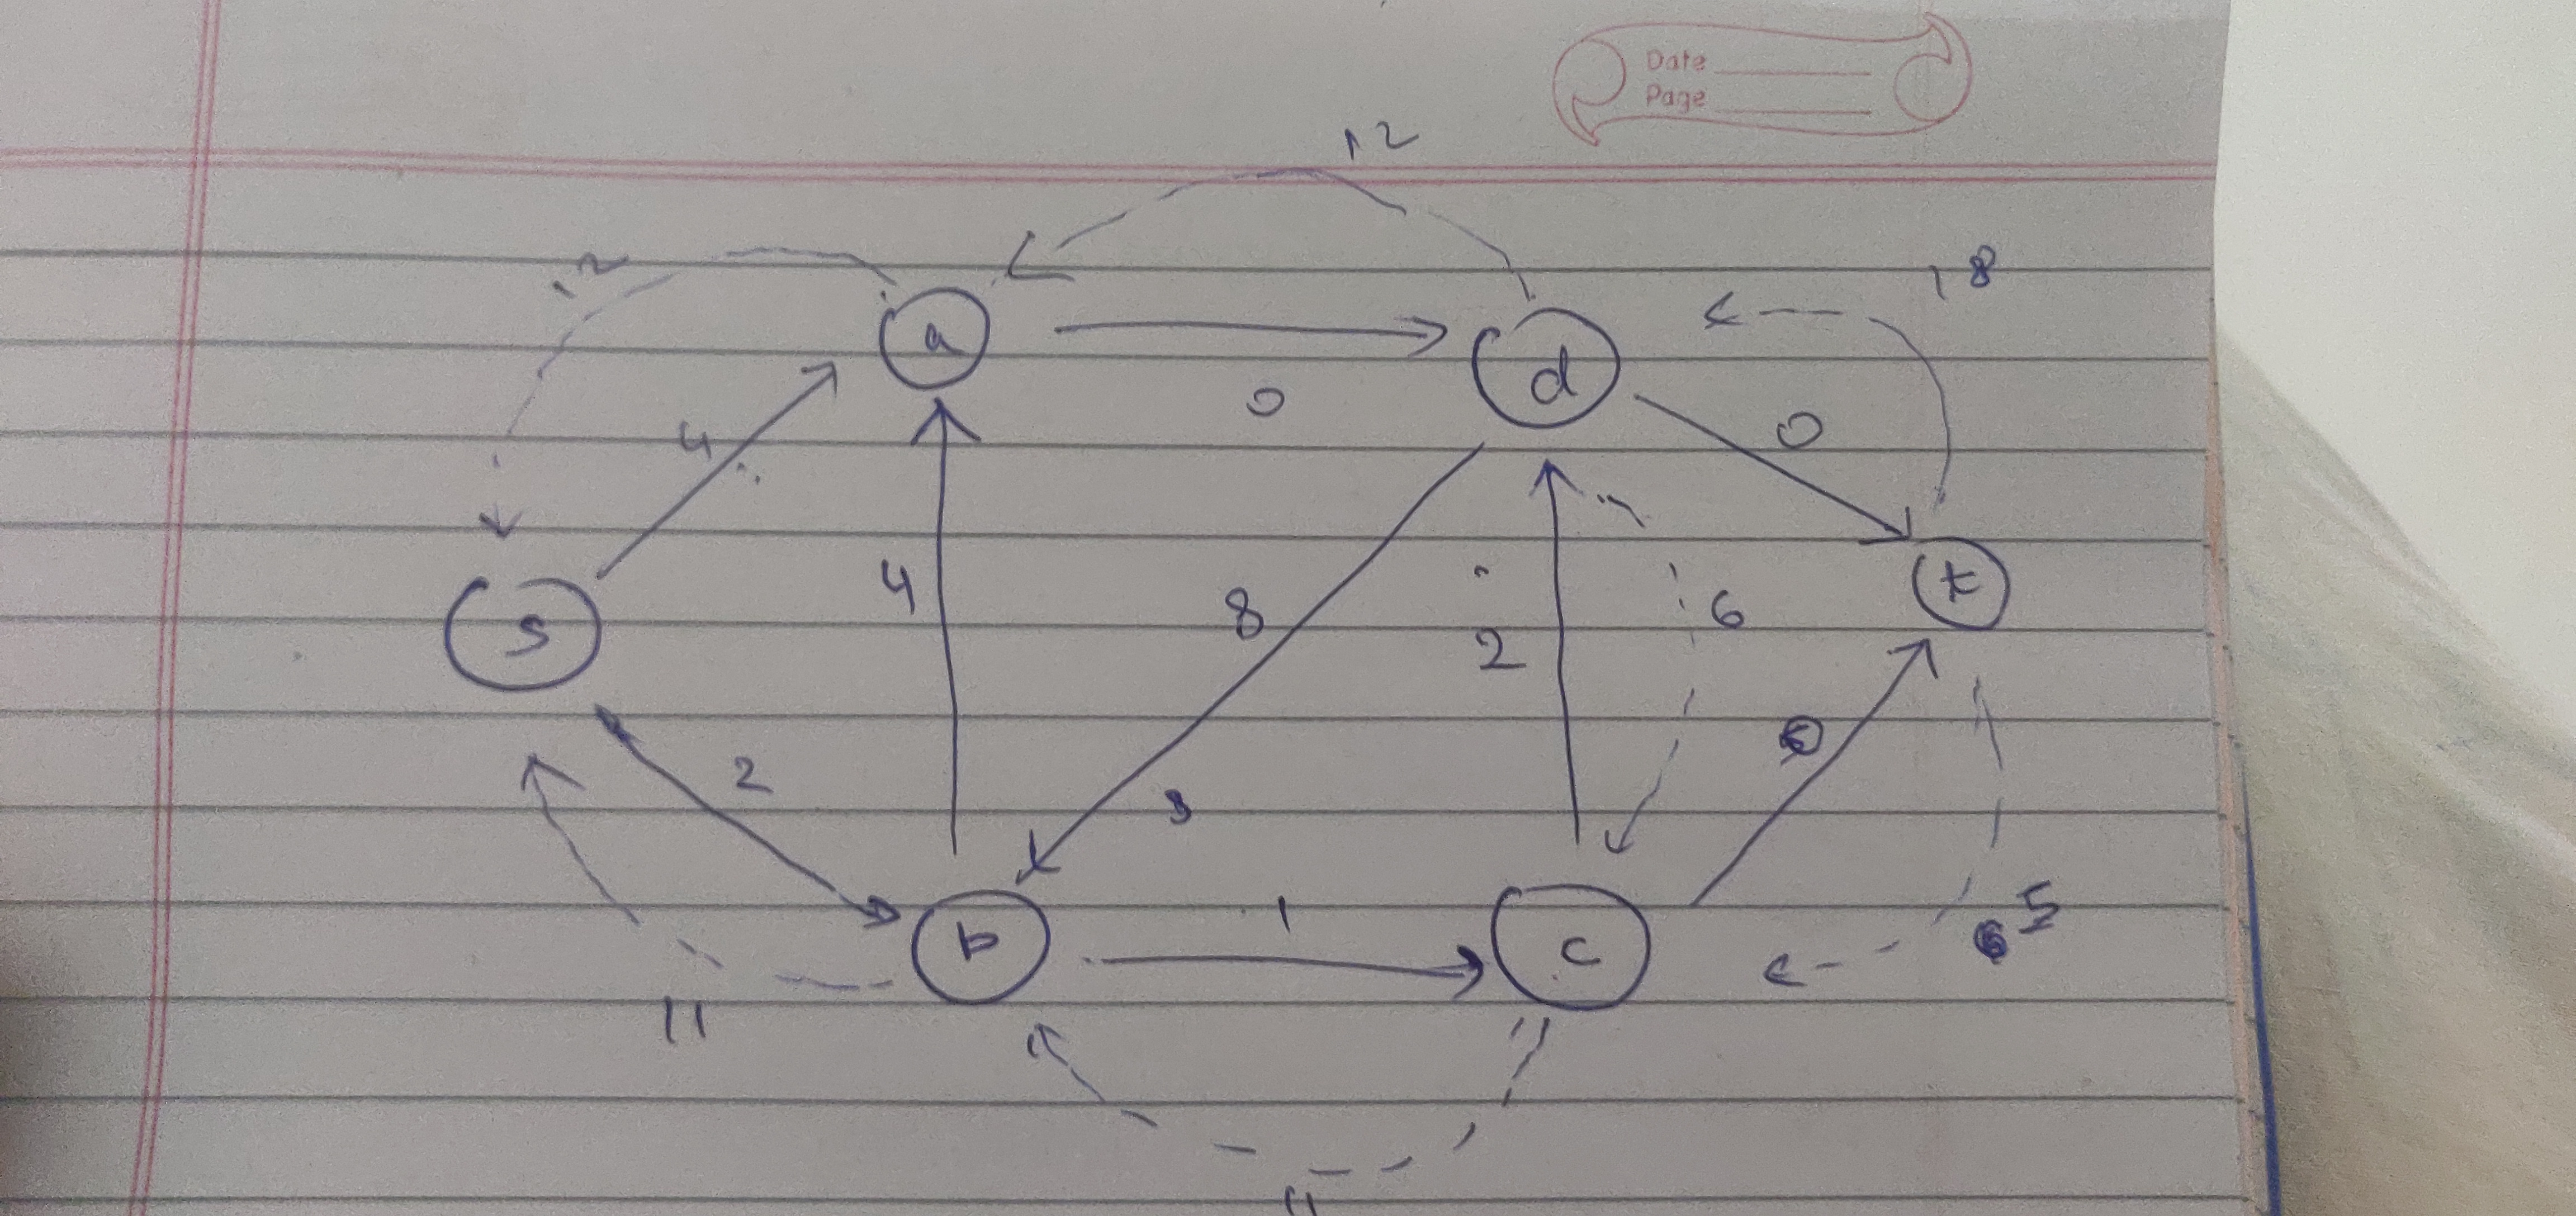
\includegraphics[scale=0.085]{1_c.jpg}
%\end{figure}

\begin{center}
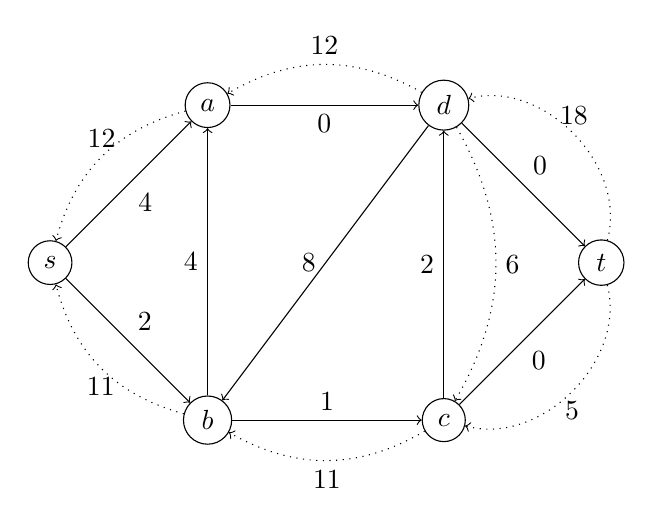
\begin{tikzpicture}
\tikzset{vertex/.style = {shape=circle,draw,minimum size=1.5em}}
\tikzset{edge/.style = {->,> = latex'}}
\node[vertex](s) at (0, 0) {$s$};
\node[vertex](a) at (2, 2) {$a$};
\node[vertex](b) at (2, -2) {$b$};
\node[vertex](c) at (5, -2) {$c$};
\node[vertex](d) at (5, 2) {$d$};
\node[vertex](t) at (7, 0) {$t$};
\draw[->] (s) -- (a) node[midway, below right] {$4$};
\draw[->] (s) -- (b) node[midway, above right] {$2$};
\draw[->] (b) -- (a) node[midway, left] {$4$};
\draw[->] (a) -- (d) node[midway, below] {$0$};
\draw[->] (d) -- (b) node[midway, left] {$8$};
\draw[->] (b) -- (c) node[midway, above] {$1$};
\draw[->] (c) -- (d) node[midway, left] {$2$};
\draw[->] (c) -- (t) node[midway, below right] {$0$};
\draw[->] (d) -- (t) node[midway, above right] {$0$};
\draw[->, dotted] (b) to [bend left] node[midway, below] {$11$} (s);
\draw[->, dotted] (c) to [bend left] node[midway, below] {$11$} (b);
\draw[->, dotted] (t) to [bend left, out=60, in=120] node[midway, below] {$5$} (c);
\draw[->, dotted] (a) to [bend right] node[midway, above] {$12$} (s);
\draw[->, dotted] (d) to [bend right] node[midway, above] {$12$} (a);
\draw[->, dotted] (t) to [bend right, out=-60, in=-120] node[midway, above] {$18$} (d);
\draw[->, dotted] (d) to [bend left] node[midway, right] {$6$} (c);
\end{tikzpicture}
\end{center}

\end{solution}

\part Give the value of the flow $f$ when the algorithm terminates. Let $A^*$ be the vertices reachable (using edges of positive weight) from $s$ in $G_f$ and let $B^*$ be the remaining vertices. Give $A^*$ and $B^*$. Give the capacity of the cut $(A^*, B^*)$.
\begin{solution}
$v(f)=23$
\newline $A^*=\{s,a,b,c,d\}$
\newline $B^*=\{t\}$
\newline $C(A^*,B^*)=\sum_{e\text{ out of }A^{*}} c(e)=18+5=23$
\end{solution}
\end{parts}






\newpage











\question Answer the following:

\begin{parts}
\part[1] \underline{State true or false}: For every $s$-$t$ network graph $G$, there is a unique $s$-$t$ cut with minimum capacity.
 
\begin{solution}
False
\end{solution}

\part[4] Give reason for your answer to part (a).

\begin{solution}
%\begin{figure}[H]
%\centering
%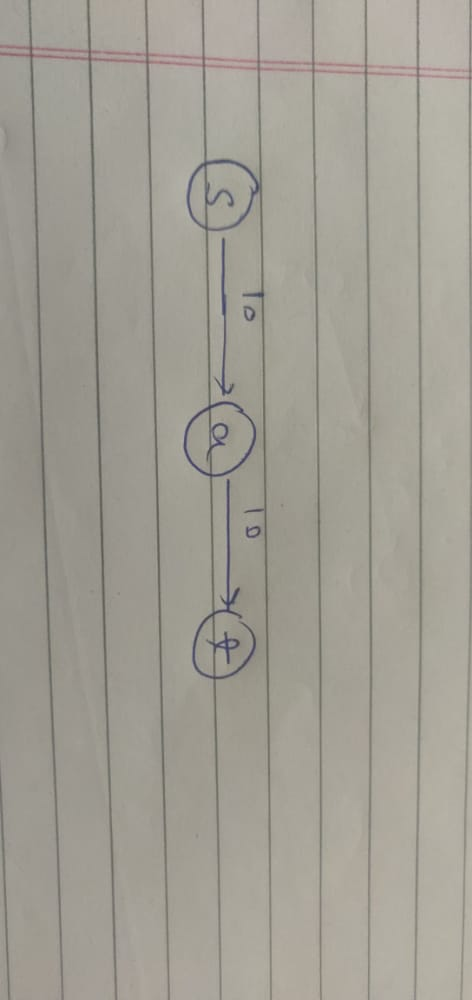
\includegraphics[height=5cm,width=10cm]{2_a.jpg}
%\end{figure}

\begin{center}
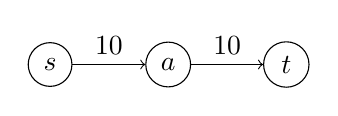
\begin{tikzpicture}
\tikzset{vertex/.style = {shape=circle,draw,minimum size=1.5em}}
\tikzset{edge/.style = {->,> = latex'}}
\node[vertex](s) at (0, 0) {$s$};
\node[vertex](a) at (1.5, 0) {$a$};
\node[vertex](t) at (3, 0) {$t$};
\draw[->] (s) -- (a) node[midway,above] {$10$};
\draw[->] (a) -- (t) node[midway,above] {$10$};
\end{tikzpicture}
\end{center}

In the above figure if we consider sets
\newline $A= \{s\}$
\newline $B= \{a,t\}$
\newline $A'= \{s,a\}$
\newline $B'= \{t\}$
\newline There are two cuts possible for the given flow: $(A,B)$ and $(A',B')$. We can see that both have capacity 10. So the minimum capacity for any cut in the network graph is 10, and there are two possible cuts with that capacity. Therefore the given statement is false.
\end{solution}
\part[1] \underline{State true or false}: For every $s$-$t$ network graph $G$ and any edge $e$ in the graph $G$, increasing the capacity of $e$ increases the value of maximum flow.

\begin{solution}
False
\end{solution}

\part[4] Give reason for your answer to part (c).
\begin{solution}
To prove that the statement is false, it is sufficient to provide a counterexample.
 
Consider the two graphs below. In the second one, the capacity of the edge $a\to t$ is changed from 10 to 20.
\newline For the first graph the maximum flow will be 10.
\newline For the second graph the maximum flow will also be 10.
\newline So despite increasing the capacity of an edge, the maximum flow remains the same, and hence this is a valid counterexample.


%\begin{figure}[H]
%\centering
%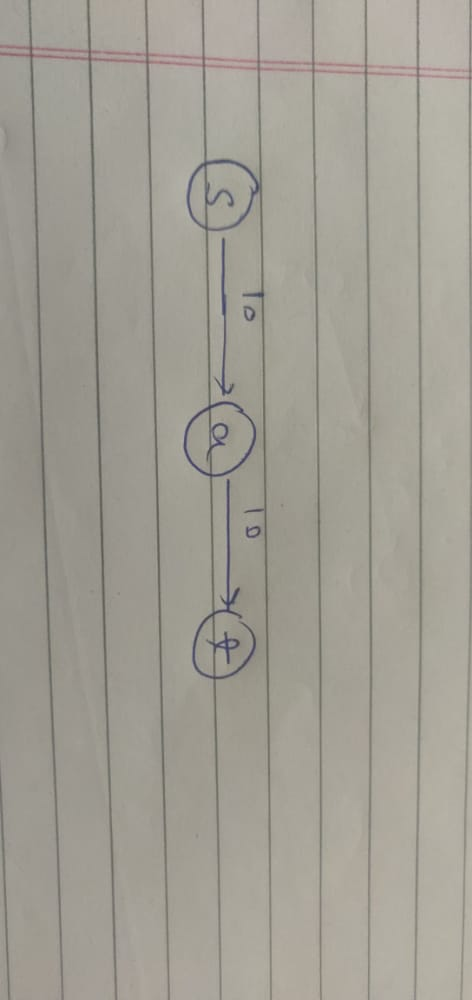
\includegraphics[height=5cm,width=10cm]{2_a.jpg}
%\end{figure}
%\begin{figure}[H]
%\centering
%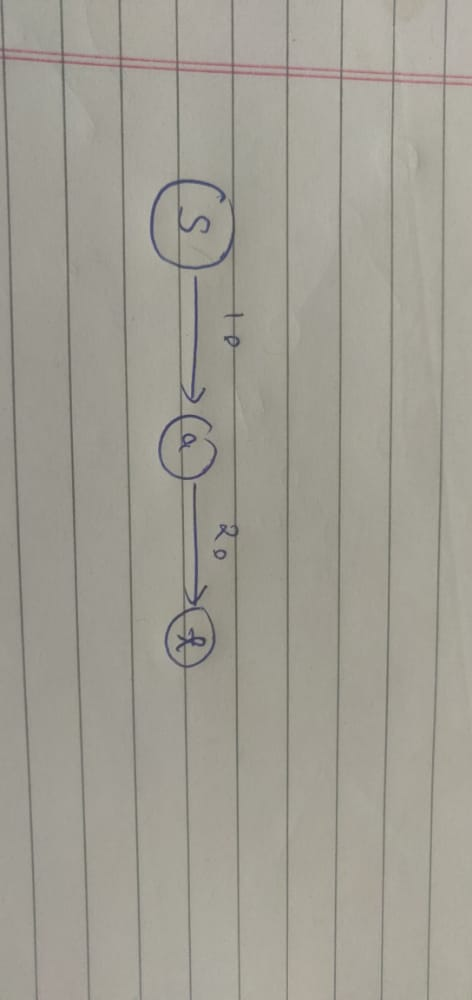
\includegraphics[height=5cm,width=10cm]{2_b.jpg}
%\end{figure}


\begin{center}
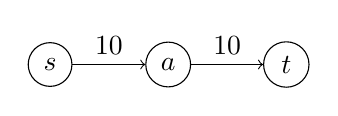
\begin{tikzpicture}
\tikzset{vertex/.style = {shape=circle,draw,minimum size=1.5em}}
\tikzset{edge/.style = {->,> = latex'}}
\node[vertex](s) at (0, 0) {$s$};
\node[vertex](a) at (1.5, 0) {$a$};
\node[vertex](t) at (3, 0) {$t$};
\draw[->] (s) -- (a) node[midway,above] {$10$};
\draw[->] (a) -- (t) node[midway,above] {$10$};
\end{tikzpicture}
\end{center}

\begin{center}
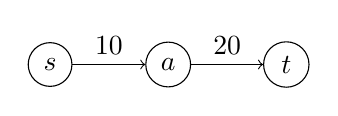
\begin{tikzpicture}
\tikzset{vertex/.style = {shape=circle,draw,minimum size=1.5em}}
\tikzset{edge/.style = {->,> = latex'}}
\node[vertex](s) at (0, 0) {$s$};
\node[vertex](a) at (1.5, 0) {$a$};
\node[vertex](t) at (3, 0) {$t$};
\draw[->] (s) -- (a) node[midway,above] {$10$};
\draw[->] (a) -- (t) node[midway,above] {$20$};
\end{tikzpicture}
\end{center}


\end{solution}

\part[1] \underline{State true or false}: For every $s$-$t$ network graph $G$ for which an $s$-$t$ flow with non-zero value exists, there exists an edge $e$ in the graph such that decreasing the capacity of $e$ decreases the value of maximum flow.

\begin{solution}
True
\end{solution}

\part[4] Give reason for your answer to part (e).

\begin{solution}
Let $A^*$ be the set of vertices reachable from $s$ in the residual graph $G_f$ corresponding to the maximum flow, and let $B^*$ be the set of the remaining vertices. Then $(A^*, B^*)$ is an $s-t$ cut.

Note that there must be at least one edge from $A^*$ to $B^*$ since otherwise, there would be no edge from $A^*$ to $B^*$ implying that the capacity of this cut is 0, which means that the maximum flow is 0, which is false by the problem condition.

Note that the capacity of this cut equals the minimum flow as done in class, say $c$. %(TODO: IS THIS OKAY TO WRITE?)

Consider any edge $e = (x, y)$ from $A^*$ to $B^*$. Reducing the capacity of this edge reduces the capacity of this cut to some $v < c$. The maximum flow value of the new graph equals the minimum cut capacity of the new graph by max-flow min-cut theorem, which can be at most $v$ since we have exhibited a cut of capacity $v$. Thus the maximum flow value of the new graph is at most $v < c$, so upon reducing the capacity of this edge, the value of the maximum flow in the graph decreases.
\end{solution}

\end{parts}

\newpage


\question Suppose you are given a bipartite graph $(L, R, E)$, where $L$ denotes the vertices on the left, $R$ denotes the vertices on the right and $E$ denote the set of edges. Furthermore it is given that degree of every vertex is exactly $d$ (you may assume that $d > 0$). 
We will construct a flow network $G$ using this bipartite graph in the following manner: $G$ has $|L| + |R| + 2$ vertices. There is a vertex corresponding to every vertex in $L$ and $R$. There is also a source vertex $s$ and a sink vertex $t$. There are directed edges with weight $1$ from $s$ to all vertices in $L$ and directed edges of weight $1$ from all vertices in $R$ to $t$. For each edge $(u, v) \in E$, there is a directed edge from $u$ to $v$ with weight $1$ in $G$.

({\it The figure below shows an example of a bipartite graph and the construction of the network.})

\begin{figure}[h]
\centering
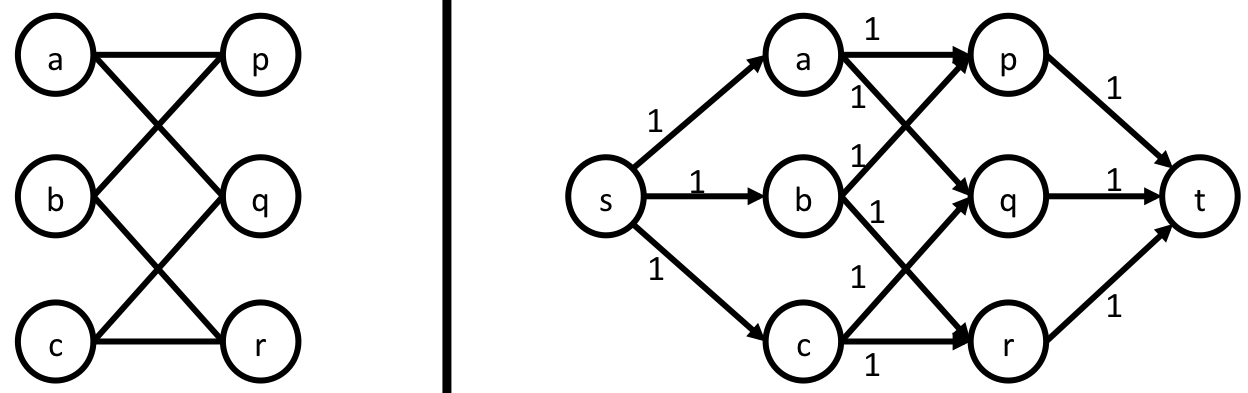
\includegraphics[scale=0.25]{embed/nf-3}
\caption{An example bipartite graph (with $d = 2$) and network construction.}
\end{figure}

\begin{parts}
\part[5] Argue that for any such bipartite graph where the degree of every vertex is equal to $d$, $|L|$ is equal to $|R|$.

\begin{solution}
We count the number of edges in two ways.

Each edge of the graph has one endpoint in $L$ and the other endpoint in $R$.

Hence, the total number of edges equals the total number of edges with exactly one endpoint in $L$, and that is precisely the sum of degrees of all vertices in the $L$ (since there is no edge between vertices in $L$), which is $d|L|$.

More formally, we have:

\begin{align*}
    \sum_{\{u, v\} \in E} 1 
    &= \sum_{(u, v) \in E \land u \in L \land v \in R} 1\\
    &= \sum_{u \in L} \sum_{(u, v) \in E \land v \in R} 1\\
    &= \sum_{u \in L} deg(u)\\
    &= \sum_{u \in L} d\\
    &= d|L|
\end{align*}

By a completely analogous argument, we have

\begin{align*}
    \sum_{\{u, v\} \in E} 1 
    &= \sum_{(u, v) \in E \land u \in L \land v \in R} 1\\
    &= \sum_{v \in R} \sum_{(u, v) \in E \land u \in L} 1\\
    &= \sum_{v \in R} deg(v)\\
    &= \sum_{v \in R} d\\
    &= d|R|
\end{align*}

Hence, we have $d|L| = d|R|$, so since $d > 0$, we have $|L| = |R|$.

\end{solution}

\part[10] Argue that for any given bipartite graph where the degree of every vertex is the same non-zero value $d$, there is an integer $s$-$t$ flow (i,e., flow along any edge is an integer) in the corresponding network with value $|L|$.

\begin{solution}
Consider any $s-t$ cut $(A, B)$. We claim that the capacity of this cut is at least $|L|$, and then exhibit a cut of capacity precisely $|L|$, to establish that the minimum capacity of a cut in the corresponding network is $|L|$, which by the max-flow-min-cut theorem equals the maximum value of a flow in the corresponding network.\nl
Let $\ell = |L| = |R|$.\nl
Note that since $(A, B)$ is an $s-t$ cut, we have $s \in A, t \in B$.\nl
Suppose $A$ has $n$ vertices from $L$ and $m$ vertices from $R$. Then $B$ has $\ell - n$ vertices from $L$ and $\ell - m$ vertices from $R$.\nl
Define $X_{IJ}$ to be the number of edges going from $L \cap I$ to $R \cap J$.\nl
Then we have $C(A, B)$ to be the number of edges from $s$ to $L \cap B$ + the number of edges from $R \cap A$ to $t$ + the number of edges going from $L \cap A$ to $R \cap B$.\nl
Hence we have $$C(A, B) = \ell - n + m + X_{AB}$$
If $n \le m$, then we are done, since then $$C(A, B) = \ell + (m - n) + X_{AB} \ge \ell + 0 + 0 = \ell$$
Now suppose $n > m$. We claim that $X_{AB} \ge n - m$.\nl
The total number of edges going from $A \cap L$ to $R$ is $X_{AA} + X_{AB}$, and it is equal to the sum of degrees of vertices in $A \cap L$, which is $dn$.\nl
Similarly, the total number of edges going from $L$ to $A \cap R$ is $X_{AA} + X_{BA}$, and it is equal to the sum of degrees of vertices in $A \cap R$, which is $dm$.
Hence we have 
\begin{align*}
X_{AB} &= X_{BA} + \left(X_{AA} + X_{AB}\right) - \left(X_{AA} + X_{BA}\right)\\
       &= X_{BA} + dn - dm\\
       &= X_{BA} + d(n - m)\\
       &\ge 0 + n - m\\
       &= n - m
\end{align*}
as needed, where the inequality comes in since $d \ge 1$ and $n > m$.
Hence in this case too, we have $C(A, B) \ge \ell$.\nl
Thus we have shown that $C(A, B) \ge \ell$ for any $s-t$ cut.

Now consider the cut where $A = \{s\}$, and $B$ is the set of the remaining vertices. Note that here the capacity of the cut is the sum of 1 over all edges outgoing from $s$, which is $\ell$.

Hence for a particular cut, we have shown that $C(A, B) = \ell$, which when combined with the previous bound shows that the minimum capacity of a cut in the network is $\ell$, and by the max-flow-min-cut theorem, this is equal to the maximum flow of the network.

Since the maximum flow of the network has value $|L|$, there exists a flow with value $|L|$, and since this flow is a maximum flow on a network with integer capacities, it can be computed using the Ford-Fulkerson algorithm, which always guarantees that the flow it returns is an integer flow. Hence there exists an integer $s-t$ flow in the corresponding network with value $|L|$, as desired.
\end{solution}

\part[5] A matching in a bipartite graph $G = (L, R, E)$ is a subset of edges $S \subseteq E$ such that for every vertex $v \in L \cup R$, $v$ is present as an endpoint of at most one edge in $S$. A maximum matching is a matching of maximum cardinality. Show that the size of the maximum matching in any bipartite graph $G = (L, R, E)$ is the same as the maximum flow value in the corresponding network graph defined as above.

\begin{solution}
We shall 
\begin{enumerate}
    \item Construct a valid flow $f$ of size $|f|$ from any valid matching of size $|f|$.
    \item Construct a valid matching of size $|f|$ from any valid flow $f$.
\end{enumerate}

\paragraph{Construction of flow from a maximum matching}
Suppose $S$ is the set of all edges in the matching. By the bipartite-ness of the graph, each edge has exactly one endpoint in $L$ and the other one in $R$. Hence, for each edge $(u, v)$, where $u \in L, v \in R$, set $f((s, u)) = f((u, v)) = f((v, t)) = 1$ in the network. In the end, set $f$ of all the remaining edges in the network to $0$.\nl
We need to show that this is a valid flow, and that the value of this flow is $|S|$.\nl
For showing that it is a valid flow, we need to show flow conservation and the satisfaction of capacity constraints.
\begin{enumerate}
    \item Flow conservation: Consider any vertex $u \in L$. If $f((s, u)) = 1$, then there must have been an edge in $S$ with $u$ as an endpoint (and exactly one such edge by the definition of a matching). Hence, $\sum_{e \text{ into } u}f(e) = 1$ and $\sum_{e \text{ out of } u}f(e) = 1$. For a vertex $u$ which has $f((s, u)) = 0$, it is not an endpoint of any edge in $S$, so $\sum_{e \text{ into } u}f(e) = 0$ and $\sum_{e \text{ out of } u}f(e) = 0$. Now consider any vertex $v \in R$. If $f((v, t)) = 1$, then there must have been an edge in $S$ with $v$ as an endpoint (and exactly one such edge by the definition of a matching). Hence, $\sum_{e \text{ into } v}f(e) = 1$ and $\sum_{e \text{ out of } v}f(e) = 1$. For a vertex $v$ which has $f((v, t)) = 0$, it is not an endpoint of any edge in $S$, so $\sum_{e \text{ into } v}f(e) = 0$ and $\sum_{e \text{ out of } v}f(e) = 0$. Hence for all internal vertices, flow conservation holds.
    \item Capacity constraints: Since we assign either $0$ or $1$ to any edge, and the capacity of an edge is $1$, the capacity constraints hold trivially.
\end{enumerate}
Now to show that the value of this flow is $|S|$, note that any edge in $S$ has exactly one endpoint in $L$, and no two edges in $S$ share an endpoint. Hence, the number of vertices with $f((s, u)) = 1$ is precisely the number of edges in $S$, which is $|S|$. However, the value of the flow is the sum of $f-$values assigned to edges emanating from $s$, which is equal to the number of edges emanating from $s$ which we assigned 1 to, and that equals $|S|$.\nl
Hence, this is a valid flow, and the capacity of the flow is $|S|$ and we are done.
\paragraph{Construction of matching from a maximum flow}
Note that in a flow network with integer capacities, the maximum value of a flow is an integer, and there exists a flow with the maximum value, such that all $f-$values of edges are integers (which can be found using the Ford-Fulkerson algorithm).\nl
Consider such a flow $f$, and the set of edges between internal nodes having $f-$values positive (and by combining the the discussion above and capacity constraints, the $f-$values must be $1$).\nl
More formally, let $S$ be the set of edges $(u, v)$ such that $f((u, v)) > 0$, and $\{s, t\} \cap \{u, v\} = \emptyset$. Then $f((u, v))$ is an integer and upper bounded by $1$, so it is $1$ for all such vertices. Note that we need to make each edge undirected before including it in $S$.\nl
We claim that $S$ is a matching with size equal to the value of the flow.
\begin{enumerate}
    \item $S$ is a matching: Note that $S$ has edges incident only on vertices which are in $G$. Hence, $S$ is a subset of $E$ by the construction of the network. Now suppose there exists a vertex $v \in L \cup R$ which is incident to at least 2 edges in $S$. We make two cases:
    \begin{enumerate}
        \item $v \in L$: In that case, we have at least two edges emanating from $v$ which have $f(e) = 1$. Hence by flow conservation, the sum of weights of all edges into $v$ must be at least $2$, which is a contradiction, since the only edge coming into $v$ is $(s, v)$, and it has capacity $1$.
        \item $v \in R$: In that case, we have at least two edges coming into $v$ which have $f(e) = 1$. Hence by flow conservation, the sum of weights of all edges emanating from $v$ must be at least $2$, which is a contradiction, since the only edge emanating from $v$ is $(v, t)$, and it has capacity $1$.
    \end{enumerate}
    Hence we have shown that $S$ is a matching.
    \item $|S| = v(f)$: Firstly note that since $G$ is bipartite, all edges in $S$ have exactly one endpoint each in $L$ and $R$. Consider the set $T$ of all vertices in $L$ that are incident to an edge in $S$. Then, since each edge in $S$ has an $f-$value of 1, and no two edges share a common endpoint (which implies at most 1 edge from $S$ is incident on a given vertex in $L$), $\sum_{e \text{ out of }u} f(e) = 1$ for each $u$ in $T$. By flow conservation, for each vertex $v$ in $T$, we have $f((s, v)) = 1$. For the remaining vertices, using the same argument, we have $f((s, v)) = 0$. Summing this over all vertices in $L$, we have $v(f) = |T|$. Now since no two edges in $S$ share an endpoint, we have $|S| = |T|$, and hence we have $|S| = v(f)$, as required.
\end{enumerate}

From here, we can see that we have constructed a flow $f$ with $v(f)$ being equal to the cardinality of the maximum matching, and also that we have constructed a matching with the cardinality being equal to the maximum value of any flow $f$.\nl
Hence, the maximum value of a flow equals the cardinality of a certain valid matching, which is at most the cardinality of a maximum matching.\nl
Also, the cardinality of a maximum matching equals the value of a certain valid flow, which is at most the maximum value of a flow.\nl
Combining these inequalities, we can see that equality holds, and thus the cardinality of a maximum matching in the graph equals the maximum value of any flow in the corresponding network, as required.
\end{solution}

\end{parts}










\newpage







\question[20] There are $n$ stationary mobile-phones $c_1, ..., c_n$ and $n$ stationary mobile-phone towers $t_1, ..., t_n$. 
The distances between mobile-phones and towers are given to you in an $n \times n$ matrix $d$, where $d[i, j]$ denotes the distance between phone $c_i$ and tower $t_j$.
It is possible for a mobile-phone $c_i$ to connect to a tower $t_j$ if and only if the distance between $c_i$ and $t_j$ is at most $D$, where $D$ is the connecting radius. 
Furthermore, at one time, a mobile-phone can connect to at most one tower and a tower can allow at most one connection. 
Your goal as a Communications Engineer is to figure out whether all mobile-phones are usable simultaneously. 
That is, whether it is possible for all mobile-phones to connect simultaneously to distinct towers. Answer the following questions.

\begin{parts}
\part Consider a simple example with 5 mobile-phones and 5 towers. Let the connecting radius be $D = 2$ miles. The distance matrix for this example is as given in Figure~\ref{fig:1}.
\begin{figure}[h]
\centering
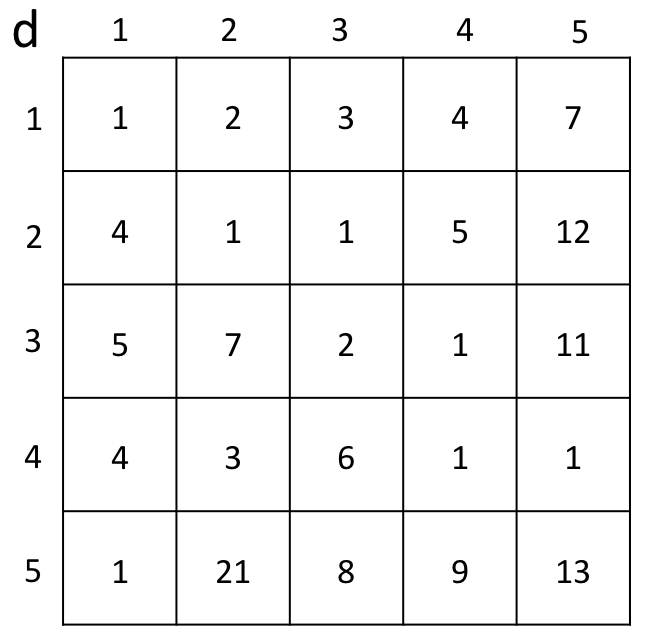
\includegraphics[scale=0.2]{embed/nf-2}
\caption{Distance matrix $d$ for part (a) of question 4.}
\label{fig:1}
\end{figure}

\underline{Prove or disprove}: It is possible for all 5 mobile-phones to simultaneously connect to distinct towers for this example.
\begin{solution}
Yes, it is possible. Here is a matching from cell-phones to towers that demonstrates how connections can be obtained.
\begin{align*}
1 &\rightarrow 2 & d[1,2]=2\\
2 &\rightarrow 3 & d[2,3]=1\\
3 &\rightarrow 4 & d[3,4]=1\\
4 &\rightarrow 5 & d[4,5]=1\\
5 &\rightarrow 1 & d[5,1]=1\\
\end{align*}
\end{solution}


\vspace{0.1in}

\part Design an algorithm that takes inputs $n$, $D$, and the distance matrix $d$, and outputs ``yes" if it is possible for all mobile-phones to simultaneously connect to distinct towers (within the connecting radius $D$) and ``no" otherwise. 
Analyze the running time of the algorithm and give proof of correctness.
\end{parts}

\begin{solution}
We will show how the given problem may be reduced to the problem of determining if there exists perfect matching in a bipartite graph. This reduction will allow us to solve the given problem using any of the algorithms for the perfect matching. 

\paragraph{Proof of Correctness}
Consider the bipartite graph $G$ with 2 partitions $X$ and $Y$ of size $n$ each. There is an edge between $X[i]$ and $Y[j]$ \emph{iff} $d[i, j] \leq D$.
An illustration of a possible graph $G$ is as shown below.
\begin{figure}[H]
    \centering
    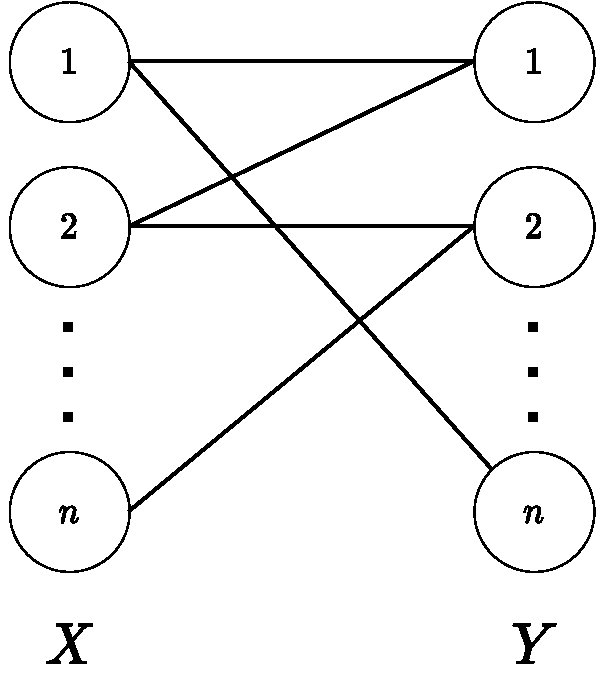
\includegraphics[width=0.3\textwidth]{embed/Bipartite1.pdf}
\end{figure}

\begin{claim}
All mobile phones will be usable simultaneously \emph{iff} there exists a perfect matching, i.e. matching of size $n$, in the bipartite graph $G$ as constructed above.
\end{claim}
\begin{proof}
We will prove this claim by proving the implication from both the sides, as follows:
\begin{claim}
Suppose that it is possible to obtain a pairing $P$ of mobile phones to the towers such that all mobile phones are usable. Then, the matching $M = \{(X[i], Y[j]) \mid (i, j) \in P\}$ is a valid matching of size $n$ in $G$.
\end{claim}
\begin{proof}
First we will show that $M \subseteq E(G)$. For this, note that if $(X[i], Y[j]) \in M$ then $(i, j) \in P$. And since $P$ is a valid pairing by assumption, we have that $d[i,j] \leq D$. Therefore $(X[i], Y[j]) \in E(G)$ by construction of $G$. Hence, $M \subseteq E(G)$. 

Note that $P$ has size $n$ by definition, since each phone is used. Now since $|M| = |P|$, we have $|M| = n$. We now only need to show that $M$ is a valid matching.
%Note that $M$ has size $n$ by definition, as $|M| = |P|$, and any valid pairing in which all mobile phones are usable must pair each mobile phone with a tower, so $|P|=n$. 

Now, suppose $M$ is not a valid matching. Then, there must be a vertex $v \in G$ such that it has more than one incident edge in $M$. Now, $v \in X$ or $v \in Y$. If $v = X[i]$ for some $i$ then it means that mobile phone $i$ is connected to more than one tower. Similarly if $v = Y[j]$ for some $j$, then it means that tower $j$ is allowing more than one connection at a time. Both of these cases violate the problem constraints and contradict the fact that $P$ is a valid pairing. Hence we must have that no such $v \in G$ can exist. Therefore, $M$ is a valid matching.
\end{proof}
\begin{claim}
Now, suppose there exists a matching $M$ of size $n$ in $G$. Then, pairing $P = \{(i, j) \mid (X[i], Y[j]) \in M\}$ of mobile phones to towers is a valid pairing such that all mobile phones are usable.
\end{claim}
\begin{proof}
Note that by definition $|P| = |M| = n$. So $P$ pairs each mobile phone to a tower. To show that $P$ is a valid pairing we need to show that if mobile phone $i$ is paired with tower $j$ then $d[i,j] \leq D$, and, each mobile phone is paired with atmost one tower and vice versa.

By definition of $P$, $(i,j) \in P$ iff $(X[i], Y[j]) \in M$. Also, by construction of $G$ if there is an edge between $X[i]$ and $Y[j]$ it implies that $d[i,j] \leq D$.

Now, if possible, let $i$ be a mobile phone that is paired with more than one tower, say $j_1, j_2$ in $P$. Then we have that $(X[i], Y[j_1]), (X[i], Y[j_2]) \in M$. But this is a contradiction because by definition a matching includes only vertex disjoint edges. \textit{Mutatis mutandis}, we can argue that all towers $j$ in $P$ will be paired with exactly one mobile phone.
\end{proof}
Hence we have proved our original claim.
\end{proof}
Using the above claim we have reduced the given problem into the problem of existence of perfect-matching in a bipartite graph $G$. So, to obtain the answer to original problem we will construct the graph $G$ as defined and then calculate the size of maximum matching in $G$. The answer will be ``yes'' \emph{iff} the size of maximum matching is $n$. The algorithm for calculating size of max-matching in a bipartite graph $G$ has already been discussed in the class using the application of network flows. So in the algorithm presented below we will assume the existence of subroutine \textsc{MaxMatching} which takes a bipartite graph $G$ and returns size of maximum matching.

\paragraph{Pseudocode}
\begin{algorithmic}[1]
\Function{ConnectionPossible}{$n$, $D$, $d$}
    \State let $X \gets $ set of $n$ nodes.
    \State let $Y \gets $ set of $n$ nodes.
    \State let $G \gets (X \cup Y, \emptyset)$
    \For {$i \in [1 \ldots n]$}
        \For {$j \in [1 \ldots n]$}
            \If{$d[i,j] \leq D$}
                \State add edge $(X[i], Y[j])$ to $G$
            \EndIf
        \EndFor
    \EndFor
    \If {\Call{MaxMatching}{$G$} $= n$}
        \State \Return ``yes''
    \Else
        \State \Return ``no''
    \EndIf
\EndFunction
\end{algorithmic}

\paragraph{Running Time Analysis}
First initialization of $G$ with no edges and $2n$ nodes will take $O(n)$ time in adjacency list representation. Then, we have a nested loop with $O(n^2)$ iterations and in each iteration we potentially add an edge to $G$. In the adjacency list representation adding an edge is equivalent to appending to the end of a linked list (or two). Therefore it will only take $O(1)$ time per iteration. So $G$ will be a graph with $2n$ vertices and at most $n^2$ edges in the worst case. \textsc{MaxMatching} algorithm routine is as discussed in the class, internally it will transform $G$ to a directed graph with $2n+2$ vertices (source and sink included) and $n^2 + 2n$ edges in the worst case. Then it will apply the ford-fulkerson algorithm to obtain the max flow in this transformed graph which will therefore take $O(n \cdot (n + n^2)) = O(n^3)$ time (since the max flow is upper bounded by $n$, and the number of vertices + edges is in $O(n + n^2)$). So overall worst case time complexity of the algorithm is $O(n^3)$.
\end{solution}

\newpage














\question[25] Town authorities of a certain town are planning for an impending virus outbreak. They want to plan for panic buying and taking cues from some other towns, they know that one of the items that the town may run out of is toilet paper. They have asked your help to figure out whether the toilet paper demand of all $n$ residents can be met. They provide you with the following information:
\begin{itemize}
\item There are $n$ residents $r_1, ..., r_n$, $m$ stores $s_1, ..., s_m$, and $p$ toilet paper suppliers $x_1, ..., x_p$.
\item The demand of each of the residents in terms of the number of rolls required.
\item The list of stores that each of the residents can visit and purchase rolls from. 
A store cannot put any restriction on the number of rolls a customer can purchase given that those many rolls are available at the store.
\item The number of rolls that supplier $x_j$ can supply to store $s_i$ for all $i \in \{1, ..., m\}$ and $j \in \{1, ..., p\}$.
\end{itemize}
The above information is provided in the following data structures:
\begin{itemize}
\item A 1-dimensional integer array $D[1...n]$ of size $n$, where $D[i]$ is the demand of resident $r_i$.
\item A 2-dimensional 0/1 array $V[1...n, 1...m]$ of size $n \times m$, where $V[i, j] = 1$ if resident $r_i$ can visit store $s_j$ and $V[i, j] = 0$ otherwise.
\item A 2-dimensional integer array $W[1...m, 1...p]$ of size $m \times p$, where $W[i, j]$ is the number of rolls of toilet paper that the supplier $x_j$ can supply to store $s_i$.
\end{itemize}

Design an algorithm to determine if the demand of all residents can be met.
That is, given $(n, m, p, D, V, W)$ as input, your algorithm should output ``yes'' if it is possible for all residents to obtain the required number of rolls and ``no'' otherwise. 
Argue correctness and discuss running time.

\vspace{0.1in}

({\it For example, consider that the town has two residents, one store and two suppliers. If $D = [2, 2], V = \begin{bsmallmatrix}1 \\ 1\end{bsmallmatrix}$, and $W = [2, 2]$, then the demand can be met. However, if  $D = [2, 2], V = \begin{bsmallmatrix}1 \\ 1\end{bsmallmatrix}$, and $W = [2, 1]$, then the demand cannot be met.})

\begin{solution}

\paragraph{Pseudocode}
\begin{algorithmic}[1]
\Function{IsRequirementMet}{$n, m, p, D, V, W$}
    \State Create source and sink vertices $s, t$
    \State Create vertices $S[1 \ldots p]$ corresponding to the suppliers
    \State Create vertices $T[1 \ldots m]$ corresponding to the stores
    \State Create vertices $R[1 \ldots n]$ corresponding to the residents
    \State Let $G$ be a graph with all the above vertices
    \For{$i \in [1 \ldots p]$}
        \State Add an edge $(s, S[i])$ with capacity $\sum_{j = 1}^m W[j, i]$ to $G$
        \For{$j \in [1 \ldots m]$}
            \State Add an edge $(S[i], T[j])$ with capacity $W[j, i]$ to $G$
        \EndFor
    \EndFor
    \For{$i \in [1 \ldots n]$}
        \State Add an edge $(R[i], t)$ with capacity $D[i]$ to $G$
        \For{$j \in [1 \ldots m]$}
            \If{$V[i, j] = 1$}
                \State Add an edge $(T[j], R[i])$ with capacity $D[i]$ to $G$
            \EndIf
        \EndFor
    \EndFor
    \If{\textsc{Value}(\Call{MaxFlow}{$G, s, t$}) $= \sum_{i = 1}^m D[i]$}
        \State \Return ``yes"
    \Else
        \State \Return ``no"
    \EndIf
\EndFunction
\end{algorithmic}

\paragraph{Proof of Correctness}

By a flow, we shall always refer to an integer flow. The max-flow returned by the function MaxFlow is always an integer flow for a flow problem with integer capacities (if we use an algorithm like the Ford-Fulkerson algorithm).

By an \textit{assignment}, we denote a tuple $(A', B')$ of arrays of size $m \times p$, $n\times m$, where $A'[i, j]$ is the number of rolls supplier $x_j$ supplies to store $s_i$, and $B'[i, j]$ is the number of rolls resident $r_i$ gets from store $s_j$, and $A', B'$ are both subject to the constraints of the problem, i.e., $0 \le A'[i, j] \le W[i, j]$, $B'[i, j] \ge 0$, and $\sum_{j = 1}^n B'[j, i] \le \sum_{j = 1}^p A'[i, j] \quad \forall i \in [1\ldots m]$.

By an \textit{efficient assignment}, we denote an assignment where the following conditions are satisfied:
\begin{align}
    \sum_{j = 1}^m B'[i, j] \le D[i] \quad \forall i \in [1\ldots n]\\
    \sum_{j = 1}^n B'[j, i] = \sum_{j = 1}^p A'[i, j] \quad \forall i \in [1\ldots m]
\end{align}

In other words, an efficient assignment is one in which we have nothing left over at a store after the residents buy rolls, and all residents take no more rolls than their requirements.

We shall first show a bijection between valid flows in the graph and efficient assignments, where if flow $f$ is mapped to the assignment $a$, then $v(f) = \sum_{i = 1}^n \sum_{j = 1}^m B'[i, j]$ (total rolls bought by residents).

\begin{proof}

Consider an efficient assignment $(A', B')$.

Consider a flow defined as follows:
\begin{enumerate}
    \item For an edge $(s, S[i])$, let the flow associated to this edge be $\sum_{j=1}^m A'[j, i]$.
    \item For an edge $(S[i], T[j])$, let the flow associated to this edge be $A'[j, i]$.
    \item For an edge $(T[j], R[i])$, let the flow associated to this edge be $B'[i, j]$.
    \item For an edge $(R[i], t)$, let the flow associated to this edge be $\sum_{j = 1}^m B'[i, j]$.
\end{enumerate}

%We note that it is possible to recover the efficient assignment from the flow uniquely too, so this mapping is an inverse.

First we show that this is a valid flow.

\begin{enumerate}
    \item Flow conservation:
        \begin{enumerate}
            \item At vertex $S[i]$: Note that the only incoming edge is $(s, S[i])$, and the only outgoing edges are $(S[i], T[j])$ for $j \in \{1\ldots m\}$. From the definition of the flow values of these edges, we are done.
            \item At vertex $T[i]$: Note that since $(A', B')$ is an efficient assignment, we have $\sum_{i = 1}^n B'[i, j] = \sum_{j = 1}^p A'[i, j]$. The only incoming edges are $(S[j], T[i])$ for $j \in \{1\ldots p\}$, and the only outgoing edges are $(T[i], R[j])$ for $j in \{1\ldots n\}$. By noting the definitions of $A', B'$ and the equality mentioned above, we are done.
            \item At vertex $R[i]$: Note that the only incoming edges are $(T[j], R[i])$ for $j \in \{1 \ldots m\}$, and the only outgoing edge is $(R[i], t)$. From the definition of the flow values of these edges, we are done.
        \end{enumerate}
    \item Capacity constraints:
        Firstly note that all weights are non-negative integers. Now for the capacity constraints, note the following:
        \begin{enumerate}
            \item For an edge $(S[i], T[j])$, the flow associated to this edge is $A'[j, i]$. By the conditions of the problem, since an efficient assignment is a valid assignment, we have $A'[j, i] \le W[j, i]$.
            \item For an edge $(s, S[i])$, the flow associated to this edge is $\sum_{j=1}^m A'[j, i]$. By summing the result of the previous case over $j$, this is $\le \sum_{j = 1}^m W[j, i]$.
            \item For an edge $(T[j], R[i])$, the flow associated to this edge is $B'[i, j]$. Since we have $B'[i, j] \le \sum_{j = 1}^n \le D[i]$ (as it is a efficient assignment), we are done for this case.
            \item For an edge $(R[i], t)$, the flow associated to this edge is $\sum_{j = 1}^m B'[i, j]$. Since we have $\sum_{j = 1}^n \le D[i]$ (as it is a efficient assignment), we are done for this case.
        \end{enumerate}
\end{enumerate}

Now we show that the value of this flow equals $\sum_{i = 1}^n \sum_{j = 1}^m B'[i, j]$. Note that by considering the $s-t$ cut $(A, B) = (V(G)\setminus\{t\},\{t\})$, since there are no edges from $B$ to $A$, we have $f^{in}(A) = 0$, so the value of the flow is $f^{out}(A) = \sum_{i = 1}^n \sum_{j = 1}^m B'[i, j]$, as needed.

Hence we have shown that for any valid assignment, there exists a valid flow in the network with value being equal to the total number of rolls bought by residents.

Now consider any flow $f$.

Consider the following assignment:

\begin{align}
    A'[i, j] = f((S[j], T[i]))\\
    B'[i, j] = f((T[j], R[i]))
\end{align}

Now we need to show that this is an efficient assignment.

\begin{enumerate}
    \item It is an assignment:\nl
    For this we need to show that $0 \le A'[i, j] \le W[i, j]$, $0 \le B'[i, j]$ and $\sum_{j = 1}^n B'[j, i] \le \sum_{j = 1}^p A'[i, j] \quad \forall i \in [1\ldots m]$.
    However, the first of these follows from the fact that $f((S[j], T[i]))$ is flow associated to an edge with capacity $W[i, j]$ in a valid flow $f$. The second of these follows from $0 \le B'[i, j]$ since it is flow associated to an edge and must be non-negative.
    The third of these follows from the fact we will show below.
    \item It is an efficient assignment:
        \begin{enumerate}
            \item Consider flow conservation applied at vertex $R[i]$. Then the total incoming flow is $\sum_{j = 1}^m f((T[j], R[i])) = \sum_{j = 1}^m B'[i, j]$, which must equal the outgoing flow. And the only outgoing edge is $(R[i], t)$ which has a capacity of $D[i]$. Hence, we must have $\sum_{j = 1}^m B'[i, j] \le D[i]$, which verifies the first condition for an assignment to be an efficient assignment.
            \item Consider flow conservation applied at vertex $T[i]$. The total incoming flow is \\$\sum_{j = 1}^p f((S[j], T[i])) = \sum_{j = 1}^p A'[i, j]$. The total outgoing flow is $\sum_{j = 1}^n f((T[i], R[j])) = \sum_{j = 1}^n B'[j, i]$. By flow conservation, this verifies the second condition for an assignment to be an efficient assignment.
        \end{enumerate}
\end{enumerate}

Now we need to show that $v(f) = \sum_{i = 1}^n \sum_{j = 1}^m B'[i, j]$.

Consider the $s-t$ cut $(A, B) = (\{s\} \cup S[1 \ldots p] \cup T[1 \ldots m], R[1 \ldots n] \cup \{t\})$.

Note that there is no edge from $B$ to $A$, so $f^{in}(A) = 0$, hence we have $v(f) = f^{out}(A)$. The only edges from $A$ to $B$ are the edges between vertices of the form $T[j], R[i]$. Hence we have $v(f) = f^{out}(A) = \sum_{i = 1}^n \sum_{j = 1}^m f((T[j], R[i])) = \sum_{i = 1}^n \sum_{j = 1}^m B'[i, j]$, as needed.

From here we see that there is a bijection between efficient assignments and valid flows in the network which have the value of the flow being equal to the total number of rolls bought by the residents in the efficient assignment.

\end{proof}

Now we shall show that if there exists an assignment which satisfies all the residents' needs, then there also exists an efficient assignment which satisfies all the residents' needs.

\begin{proof}
Consider any assignment $(A', B')$ which satisfies all the residents' needs. We shall construct an efficient assignment that also satisfies all the residents' needs using the following algorithm (note that this algorithm is never run in the final algorithm, and we aim to use this as an aid in a proof of the claim above):

\begin{algorithmic}[1]
    \Require{$\sum_{j = 1}^m B'[i, j] \ge D[i] \quad \forall i \in [1 \ldots n]$}
    \Require{$0 \le B'[i, j] \quad \forall (i, j) \in [1 \ldots n] \times [1 \ldots m]$}
    \Require{$0 \le A'[i, j] \le W[i, j]$}
    \Require{$\sum_{j = 1}^n B'[j, i] \le \sum_{j = 1}^p A'[i, j] \quad \forall i \in [1\ldots m]$}
    \Function{GetEfficientAssignment}{$A', B'$}
        \State let $A'' \gets A, B'' \gets B$
        \For{$i \in [1\ldots n]$}
            \While{$\sum_{j = 1}^m B''[i, j] > D[i]$}
                \State $j = \argmax_{j} B''[i, j]$
                \State $B''[i, j] \gets B''[i, j] - 1$
            \EndWhile
        \EndFor
        \For{$i \in [1\ldots n]$}
            \While{$\sum_{j = 1}^n B''[j, i] < \sum_{j = 1}^p A''[i, j]$}
                \State $j = \argmax_{j} A''[i, j]$
                \State $A''[i, j] \gets A''[i, j] - 1$
            \EndWhile
        \EndFor
        \State \Return $(A'', B'')$
    \EndFunction
\end{algorithmic}

We claim that the above algorithm returns an efficient assignment that also satisfies the demands of all residents.

\begin{enumerate}
    \item It is an assignment
        \begin{enumerate}
            \item $B''[i, j] \ge 0$: Note that we have $D[i] \ge 0$, and hence we decrement some $B''[i, j]$ if the sum of $B''[i, j']$ over all $j'$ is positive. Note that the maximum $B''[i, j']$ must be always positive (if not, then the whole sum is non-positive). Hence we decrement a $B''[i, j]$ by 1 in a step only if it is positive. This implies that once we reach zero (which we reach since $B''$ is an integer matrix and the element we decrement decreases by exactly 1 at each decrement), we never decrement it further, proving this part.
            \item $0 \le A''[i, j] \le W[i, j]$: The second part follows from the fact that $A'[i, j] \le W[i, j]$ and we either keep the value the same or decrease it. 
            For the first part, note that from the previous point, we have $\sum_{j = 1}^n B''[j, i] \ge 0$. By a completely analogous argument as in the previous point, we decrement $A''[i, j]$ only if it is positive, and hence we are done for this part.
            \item $\sum_{j = 1}^n B''[j, i] \le \sum_{j = 1}^p A''[i, j]$: We claim that equality in fact holds, and that is done in the next part.
        \end{enumerate}
    \item It is an efficient assignment
        \begin{enumerate}
            \item $\sum_{j = 1}^m B''[i, j] \le D[i] \quad \forall i \in [1\ldots n]$:
                There is a stronger assertion in the next point about satisfaction of all residents, and it is that equality holds, so we defer this to the next point.
            \item $\sum_{j = 1}^n B''[j, i] = \sum_{j = 1}^p A''[i, j] \quad \forall i \in [1\ldots m]$:
                Either the loop runs, or the first condition is false. Since we never increment $B''[i, j]$, we have $\sum_{j = 1}^n B''[j, i] \le \sum_{j = 1}^n B'[j, i]$. By the condition that stores can't supply more than the suppliers supply them, we have $\sum_{j = 1}^n B''[j, i] \le \sum_{j = 1}^n B'[j, i] \le \sum_{j = 1}^p A'[i, j]$. Hence if the loop doesn't run, we have $\sum_{j = 1}^n B''[j, i] = \sum_{j = 1}^p A'[i, j] = \sum_{j = 1}^p A''[i, j]$.
                In the case that the loop runs, we keep decrementing the value of $\sum_{j = 1}^p A''[i, j]$ by precisely $1$ in each step, till we reach a value $\le \sum_{j = 1}^n B''[j, i]$. Since $A'', B''$ are integer matrices, the value we reach is precisely $\sum_{j = 1}^n B''[j, i]$, and we are done.
        \end{enumerate}
    \item It satisfies the demands of all residents, i.e., $\sum_{j = 1}^m B''[i, j] = D[i] \quad \forall i \in [1\ldots n]$:
    Note that by the condition that the input assignment must satisfy the demands of all the residents, the loop must either run, or we have $\sum_{j = 1}^m B''[i, j] = D[i]$ already. If the loop runs, we keep decrementing the value of $\sum_{j = 1}^m B''[i, j]$ by $1$ in each step, till we reach a value $\le D[i]$. Since $B''$ is an integer matrix, the value we reach is precisely $D[i]$.
\end{enumerate}
From the above analysis, we have proven the claim, as required.
\end{proof}

Hence from here, we get that we only need to search for an efficient assignment that satisfies the needs of all residents, and by the bijection, this is equivalent to searching for a flow which satisfies all the demands.

Using the cut $(A, B) = (V(G) \setminus \{t\}, \{t\})$, noting that $f^{in}(A) = 0$ (since there is no edge from $B$ to $A$), the value of a flow $f$ in the network is $f^{out}(A)$. The capacity of this cut is $\sum_{i = 1}^n D[i]$, so we have $\textsc{Value}(\textsc{MaxFlow}(G, s, t)) = f^{out}(A) \le \sum_{i = 1}^n D[i]$, where equality holds iff all the edges $(R[i], t)$ have flow through them equal to the capacity of that edge. By considering the efficient assignment corresponding to the maximum flow, we have the fact that there exists an efficient assignment that can satisfy all residents if and only if $\textsc{Value}(\textsc{MaxFlow}(G, s, t)) = \sum_{i = 1}^n D[i]$.

Now we argue as follows:
\begin{enumerate}
    \item If there exists an assignment satisfying all residents, then there exists an efficient assignment satisfying all residents, and such an assignment is detected by the algorithm and we return ``yes".
    \item If we return ``yes", then there is an efficient assignment satisfying all residents, and since an efficient assignment is an assignment, there is an answer to the problem.
\end{enumerate}

Hence, we return ``yes" if and only if there is a solution to the problem, and ``no" in the other case (i.e., when there is no solution to the problem).

\paragraph{Time Complexity Analysis}
Consider the cuts $(\{s\}, V(G) \setminus \{s\})$, $(V(G) \setminus \{t\}, \{t\})$. Both of these cuts have capacities at least the maximum flow in the graph, from the max-flow-min-cut theorem.
Hence the maximum flow is upper bounded by 

$$C = \min \left(\sum_{i = 1}^n D[i], \sum_{i = 1}^p \sum_{j = 1}^m W[j, i]\right)$$

The number of vertices in the graph is $2 + p + m + n$, and the number of edges is $p + pm + mn + n$. 

Hence the call to $\textsc{MaxFlow}$ takes $O((1 + p + m + n + pm + mn)C)$ time, where $C$ is defined as above. The call to the value function takes $O(1 + p + m + n + pm + mn)$ time (the total number of edges and vertices in the graph).

Creating the whole graph takes $O(1 + p + m + n + pm + mn)$ time as well (apart from the computations used for computing the capacities of edges $(s, S[i])$, and checking if $(T[j], R[i])$ needs to be added or not).

For computing the capacities of the edges, the sum can be computed in $O(pm)$ time and the checks for $V[i, j]$ happen in $O(mn)$ time, so the total graph construction time is again in $O(1 + p + m + n + pm + mn)$.

Computing the total sum of demands takes time $O(m)$.

Hence the overall time complexity is $O((1 + p + m + n + pm + mn)(C + 1))$, where $C$ is defined as $C = \min \left(\sum_{i = 1}^n D[i], \sum_{i = 1}^p \sum_{j = 1}^m W[j, i]\right)$.


\end{solution}

\end{questions}
\end{document}
